\chapter{State of the art on Brain Tumor Detection methods}

\section{Introduction}
This chapter reviews the significant literature connected to this study,
which aims to establish a conceptual information system framework for
medical imaging employing MRI brain tumor pictures. The review focuses on
the use of accessible current electronic scanners, computer-based
methodologies, and their application to enhance the MRI brain tumor tissue
analysis with a comparable accuracy to manual analysis methodology.

\section{Literature Review}
In this section, we will discuss the existing literature on the
application of machine learning and deep learning techniques in the field of brain tumor detection.

\subsection{Medical Imagery}
Medical imaging is a technique that allows us to visualize the internal structure of a human body in order to diagnose various medical conditions.
\subsubsection{Existing available approaches to analyze tissues}
The routine examination of tissues is required to investigate the manifestations of the disease. With the availability of the medical images now, it provides a great opportunity to visualize tissue samples in order to diagnose various medical conditions. In order to make this diagnosis, there are three possible ways to perform this examination in the laboratory, including:

\begin{enumerate}
  \item Traditional microscopic analysis.
  \item Capturing the images using electronic devices and Analysis.
  \item Computer based approaches using digitized images.
\end{enumerate}

\subsubsection{Traditional microscopic analysis}
In the histopathology laboratory, professionals analyze slides of biopsy
specimens using a microscope for counting and identification of different
kinds of tissues. says that normally sample tissues acquired from a biopsy
is cut into small segments (often 5 – 20 microns), processed and put onto
glass slides. In addition to that preservation and staining is a component
of processing the tissue segment in the fabrication of histopathology slides.
34

Generally, pathology professionals then conduct out manual inspection of these slides using a microscope as a regular job at different magnification levels (e.g. 10x, 20x, 40x, 100x, 200, 400x) to make judgements. Typically, histopathology slides are more informative than other modalities.

With advancements in computer power and the development of digital
scanners and image processing tools, digital histopathology image analysis
enables specialists to augment to help analyze the pictures. This decreases
the time and effort necessary for diagnosis by pathologists as well as reduces
human error and subjectivity. There are numerous sorts of digital scanners
accessible at today to study various types of tissue structures which include
Ultrasound, CT, MRI, PET.
\subsubsection{Capturing the images using electronic devices}
From what we mentioned, ultrasound despite its wide fame in the field
of medical imaging and its low risk to patients. However, it is limited from
the side that it cannot treat small tissues, as it is only specialized for large
tissues. Compared to ultrasound, the use of CT and MRI delivers better
when considering cancer tissues especially brain tumors and among CT
and MRI. Among CT and MRI, MRI provides greater soft tissue contrast
than other techniques because it can present in detail and can distinguish
tissues in the brain. MRI are considered safe for patients to avoid harmful
effects because they do not use ionizing radiation during the examination,
and provide more detail than CT images.
\subsubsection{Computer-Aided methods using digitized images obtained from biopsy
  specimen slides}
Manual microscopic examination is time intensive, prone to mistakes
and produces uneven results among specialists. Most utilized electronic
scanner like ultrasound can only detect big and mature follicles. Additionally, CT, MRI and UT need professionals’ assistance. To solve the
challenges connected with microscopic analysis and electronic scanners
computer-based techniques would be a feasible solution since computerized
image analysis minimizes time, effort, human mistakes and subjectivity for
the diagnosis of diverse tissues by pathologists. There are several sorts of
35current computer-based methodologies accessible at present which largely
considers cancer tissue analysis, blood vessel analysis and lymphatic channel analysis. While there are so many current ways accessible to date yet
none of the present approaches are suited to evaluate MRI brain tumor
tissues. This is owing to the fact that none of the available systems are totally automated which do not need any human interaction when assessing
a fresh batch of photographs.
\begin{figure}[H]
  \centering
  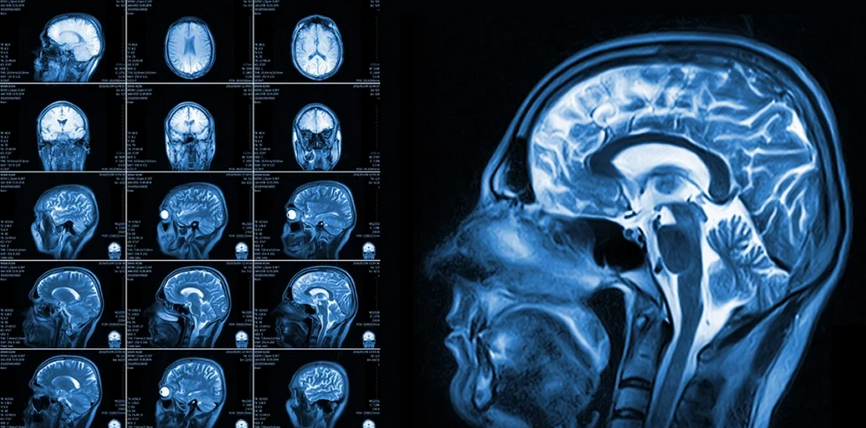
\includegraphics[width=0.7\textwidth]{Images/Chapter1/mri.png}
  \caption{Example of brain MRI image. \cite{sjra2023brainmri}}
  \label{fig:mri}
\end{figure}
\subsection{Image processing techniques}

\subsubsection{Image Pre-processing}
The medical images processed contain a great deal of information as
they are usually noisy due to unwanted pixels. it is always necessary to preprocess as a first step in most current image analysis techniques to analyze
the image of the brain tumor where pre-processing aims to improve:

\begin{enumerate}
  \item \textbf{Noise removal}: Removing impulse noise from images is one of the most important concerns in digital image processing, where noise must be removed in a way that preserves the important information of the image. A variety of techniques are used to eliminate and reduce noise in images, including a Gaussian filter, which is used to remove details and noise. It provides positive and enhanced results for noisy images.
  \item \textbf{Enhance contrast}: It is defined as the manipulation and redistributing the image pixels in a linear or non-linear fashion to improve the separation of obscured structural variations in pixel intensity into a more visually differentiable structural distribution \cite{yadav2020image}. However, there is no universal theory for enhance contrast approach \cite{nishu2012quantifying}. Digitized images acquired from MRI are typically grayscale images. It is hard to deal with the intensity of a grayscale image straightway \cite{nishu2012quantifying}. The processing of contrast enhancement histograms is one of the most widely used approaches. The processing of histogram includes equalization (An approach that extends the intensity range and improves image contrast.) and normalization (An approach for modifying the series of pixel intensity values according to relative frequencies).
\end{enumerate}

\subsubsection{Segmentation}
Segmentation is the most important part in image processing. Fence
off an entire image into several parts which is something more meaningful
and easier for further process. These several parts that are rejoined will
cover the entire image. Segmentation may also depend on various features
that are contained in the image. It may be either color or texture. Before
denoising an image, it is segmented to recover the original image. The
main motto of segmentation is to reduce the information for easy analysis.
Segmentation is also useful in Image Analysis and Image Compression \cite{yogamangalam2013segmentation}.

\subsubsection{classification}
Although there are many techniques used to identify and classify each
depending on the characteristics they target for detection, for images of
MRI brain tumor, there are three basic characteristics (shape, size, and
color) required for tumor detection. In most cases, the svm algorithm is
used, but more recently, the Convolutional Neural Network approach is
also widely used in medical image processing.

\subsubsection{Detection}
Image detection is a technique that analyzes the picture and finds
items inside it, medical image detection refers to the process of recognizing
medical-related objects that are included within an image. This assists in
establishing the precise placement of multiple tissues as well as the direction
of those tissues.

\section{Related Work}
\label{sec:related-work}


In this section, we review key approaches to brain tumor segmentation and classification that motivated our work. We focus on five representative studies, highlighting their main techniques and results, and then summarize them in Table~\ref{tab:related-work-summary}.

\subsection{Brain Tumor Segmentation and Grading of Lower‑Grade Glioma}
Naser \emph{et al.}~\cite{naser2020glioma} used a U‑Net–based CNN with transfer learning from VGG16 to segment tumors in 110 T1‑FLAIR cases of low‑grade glioma (LGG). They then classified LGG into grade II vs III, achieving 89\,\% accuracy on slice‑level MRI and 95\,\% at the patient level. In contrast, our work employs transfer learning to distinguish among three tumor types rather than grades, and omits mask‑based classification in favor of position and texture cues.

\subsection{Wavelet Statistical Texture + \glsxtrshort{rnn} }
Begum \emph{et al.}~\cite{begum2020wavelet} combined optimal wavelet statistical features with an RNN classifier. Their pipeline includes Gaussian filtering for noise removal, OGSA‑based feature selection, RNN classification, and tumor ROI segmentation via a modified region growing algorithm (MRG). They reported 95\,\% accuracy. Our approach instead uses skull stripping with morphological dilation/erosion (and GrabCut verification) to eliminate noise without explicit filtering.

\subsection{Hybrid CNN + \glsxtrshort{nade}}
Hashem \emph{et al.}~\cite{hashem2020nade} trained two parallel CNNs whose feature outputs are combined via a Neural Autoregressive Distribution Estimator (NADE). This joint distribution aids in tumor shape identification. Using cross‑entropy loss on 3\,064 T1‑weighted images (6‑fold CV), they achieved 95\,\% accuracy. We similarly verify segmentation masks with GrabCut, but replace NADE’s distribution estimation with model‑derived morphological consistency checks.

\subsection{Hierarchical Transfer Learning with AlexNet \& GoogleNet}
The framework in~\cite{kulkarni2020framework} applies skull stripping and then uses AlexNet to classify tumors into benign vs malignant, followed by GoogleNet to further distinguish malignant into glioma vs meningioma. With data augmentation (flips, rotations), they report:
\begin{itemize}
  \item Benign vs Malignant: precision 93.75\,\%, recall 100\,\%, F1 96\,\%.
  \item Glioma vs Meningioma: precision 95\,\%, recall 100\,\%, F1 97.43\,\%, accuracy 97.50\,\%.
\end{itemize}
Our demo uses a single‑stage classifier for three tumor types, with GrabCut–verified skull stripping to preserve T1‑FLAIR properties.

\subsection{VGG Block‑wise Fine‑Tuning}
Lee \emph{et al.}~\cite{swati2019transfer} employ VGG19 with a block‑wise fine‑tuning strategy, dividing the network into six blocks and progressively unfreezing from the last block. Evaluated on the same 3\,064 T1‑weighted set (5‑fold CV), they reach 94.42\,\% accuracy. We adopt transfer learning as well but use discriminative slanted triangular learning rates rather than linear schedules for fine‑tuning.

\begin{table}[ht]
  \centering
  \caption{Summary of prior methods in brain tumor segmentation and classification}
  \label{tab:related-work-summary}
  \begin{tabular}{p{0.22\textwidth} p{0.24\textwidth} p{0.16\textwidth} p{0.28\textwidth}}
    \hline
    \textbf{Study}                                             & \textbf{Approach} & \textbf{Dataset} & \textbf{Key Results} \\
    \hline
    \vspace{0.1cm} Naser \emph{et al.}~\cite{naser2020glioma}  &
    \vspace{0.1cm} U-Net + VGG16 transfer learning             &
    \vspace{0.1cm} 110 LGG (T1‑FLAIR)                          &
    \vspace{0.1cm} MRI accuracy: 89\%, patient accuracy: 95\%                                                                \\
    \hline
    \vspace{0.1cm} Begum \emph{et al.}~\cite{begum2020wavelet} &
    \vspace{0.1cm} OGSA wavelet + RNN + MRG segmentation       &
    \vspace{0.1cm} BraTS2020 (?)                               &
    \vspace{0.1cm} 95\% accuracy                                                                                             \\
    \hline
    \vspace{0.1cm} Hashem \emph{et al.}~\cite{hashem2020nade}  &
    \vspace{0.1cm} Hybrid CNNs + NADE                          &
    \vspace{0.1cm} 3,064 T1-weighted images                    &
    \vspace{0.1cm} 95\% (6-fold CV)                                                                                          \\
    \hline
    \vspace{0.1cm} Framework~\cite{kulkarni2020framework}      &
    \vspace{0.1cm} AlexNet $\to$ GoogleNet hierarchy           &
    \vspace{0.1cm} BraTS2020 (?)                               &
    \vspace{0.1cm} Benign vs Mal: F1 96\%;
    \vspace{0.1cm} Glioma vs Men: F1 97.43\%, acc 97.50\%                                                                    \\
    \hline
    \vspace{0.1cm} Lee \emph{et al.}~\cite{swati2019transfer}  &
    \vspace{0.1cm} VGG19 block-wise fine-tuning                &
    \vspace{0.1cm} 3,064 T1-weighted images                    &
    \vspace{0.1cm} 94.42\% (5-fold CV)                                                                                       \\
    \hline
  \end{tabular}
\end{table}

\section{Conclusion}
In this chapter, we reviewed key approaches to brain tumor segmentation and classification, highlighting the most utilized machine learning and deep learning models for this purpose. We examined studies that informed our work, focusing on their methodologies and results.
